\chapter{Related Work} \label{chap:Chapter3}       
\epigraph{``This is where technology is now, imagine where we can go in the future” }{\textit{Timothy Chung}}

Σε αυτό το \emph{Chapter} περιγράφονται τρόποι - από την βιβλιογραφία - με τους οποί\-ους, οι υπάρχουσες εφαρμογές 
από drone swarms επιλύουν το localization pro\-blem. Κάποια από τα συστήματα στις υπάρχουσες έρευνες\udot έχουν καθαρά
θεωρητική πλευρά, άλλα έχουν δοκιμαστεί σε real-life scenarios.
Ενώ, σε αρκετές από αυτές τις εφαρμογές χρησιμοποιούνται - 
και για αυτό γίνεται αναφορά - τεχνικές που αναφέ\-ρθηκαν στο \emph{Chapter} \ref{chap:Chapter2}.

Κυρίως, αυτά που θα μελετήσουμε θα αφορούν Cooperative Localization (\hyperref[abbr:CL]{CL}) των \hyperref[abbr:UAV]{UAV}s, ενώ επίσης
μας ενδιαφέρουν τα Distributed Computation - Real Time Location System (\hyperref[abbr:RTLS]{RTLS}) \cite{rtls}. Το πρόβλημα του Local Positioning System 
(\hyperref[abbr:LPS]{LPS}) \cite{lps} έχει ερευνηθεί από διάφορες οπτικές\udot οι οποίες μπορεί να βασίζονται σε 
\hyperref[abbr:RF]{RF}, sound waves ή ακόμα και να είναι image oriented.

Σχεδόν βέβαιο είναι επίσης, ότι από όποια κατεύθυνση και αν προσεγγίσουμε το \hyperref[abbr:LPS]{LPS} να έχουμε την ανάγκη να 
χρησιμοποιήσουμε κάποια τεχνική για να συνενώσουμε όλες τις πληροφορίες που έχουμε από τους διάφορους αισθητήρες για κάθε μεμονωμένο 
time-frame. Την ανάγκη αυτού έρχεται να καλύψει η έννοια του \emph{sensor fusion} \cite{sensor-fusion}, με μερικούς γνωστούς 
αλγόριθμους που να το επιτυγχάνουν - να είναι το  
Extended Kalman Filter (\hyperref[abbr:EKF]{EKF}), Unscented Kalman Filter (\hyperref[abbr:UKF]{UKF}), Covariance Intersection  
Filter (\hyperref[abbr:CIF]{CIF}),  Split  Covariance  Intersection  Filter (\hyperref[abbr:SCIF]{SCIF}) και  Belief  Propagation 
(\hyperref[abbr:BP]{BP}) \cite{fusion-filters}. 

Τέλος, είναι επίσης σημαντικό να αναφερθούν τα βασικά \emph{coordinate frames} τα οποία χρησιμοποιούνται. 
Αισθητήρες όπως το \hyperref[abbr:IMU]{IMU} και το compass κάνουνε μετρήσεις με γνώμονα το ίδιο το σώμα 
του αντικειμένου για αυτό - σε αυτήν την περίπτωση το σύστημα αξόνων ονομάζεται body frame (B frame) \cite{uwb-imu-gps1}.
Συχνά είναι όμως βολικό να μετατρέψουμε αυτές τις μετρήσεις σε ένα κοινό North East Down (\hyperref[abbr:NED]{NED}) 
σύστημα, οπότε τότε αναφερόμαστε σε N frame \cite{uwb-imu-gps1} \cite{body-frames}. Παράδειγμα μεταξύ των δύο 
συστημάτων βρίσκεται στο \emph{Figure} \ref{fig:Important-coordinate-frames}.

\begin{figure} [H]
	\centering
	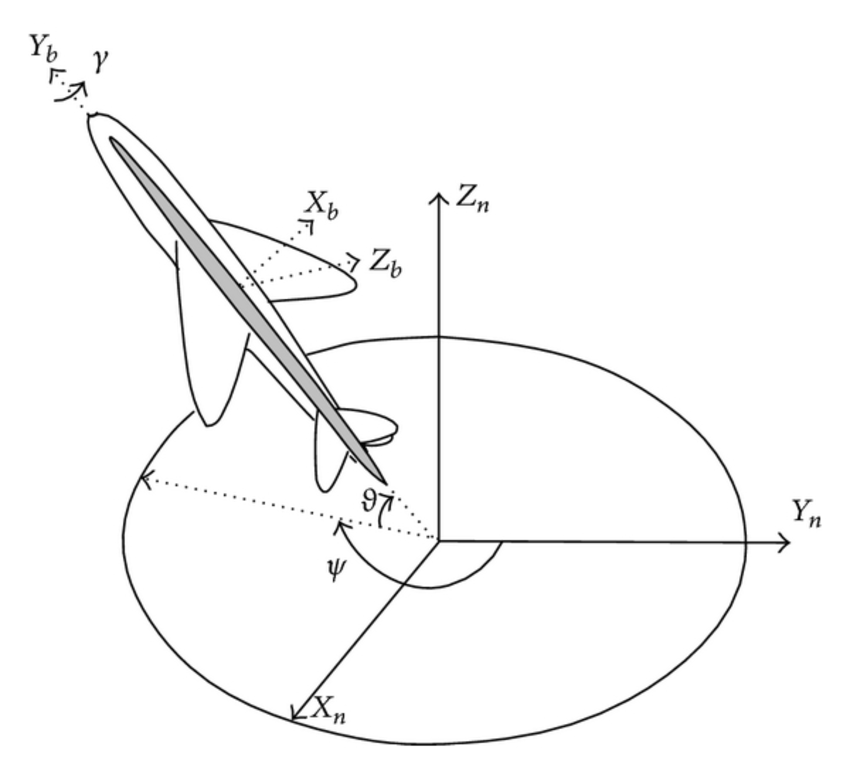
\includegraphics[width=0.6\linewidth]{Images/Related-Work/b-frame-n-frame-and-Euler-angles.png}
	\decoRule
	\caption[Important coordinate frames]{Important coordinate frames \cite{body-frames}}
	\label{fig:Important-coordinate-frames}
\end{figure}


% ------------------------------------------------------------------------------------
\section{Radio Frequency}
Το πιο εύκολο που μπορούμε να φανταστούμε είναι να χρησιμοποιήσουμε \hyperref[abbr:RF]{RF} τε\-χνο\-λο\-γίες
όπως WiFi, Zigbee και Ultra-Wideband (\hyperref[abbr:UWB]{UWB}) για την επικοινωνία και την υλοποίηση του \hyperref[abbr:LPS]{LPS}.   
Το WiFi είναι εύκολα προσβάσιμο\udot με μικρό κόστος ενώ το Zigbee προτιμάται για
low power consumption εφαρμογές. Όμως προβλήματα αυτών των δύο είναι, ότι το 
WiFi έχει μικρή εμβέλεια\footnote{Αυτό είναι κυρίως πρόβλημα για outdoor scenarios} όπως επίσης είναι πολύ εύκολο 
να υπάρχουν παρεμβολές από τις υπόλοιπες γειτονικές συσκευές\footnote{Αυτό είναι κυρίως πρόβλημα για indoor scenarios} 
άρα δεν το καθιστά καλή λύση για swarms. Το Zigbee επιλύει κάποια από αυτά τα 
προβλήματα\footnote{Σε indoor σενάρια παραμένει η δυσκολία για collision-free formation}. Συχνότερη εφαρμογή έχουν 
τα \hyperref[abbr:UWB]{UWB} καθώς επιλύει θέματα σχετικά με την ακρίβεια των μετρήσεων, το κόστος καθώς και την 
εμβέλεια\udot ταυτόχρονα \cite{uwb-imu-gps3}. Τέλος, με την χρήση του \hyperref[abbr:UWB]{UWB} επίσης, μπορούμε εύκολα να δημιουργήσουμε
ένα Flying Ad-hoc Network (\hyperref[abbr:FANET]{FANET}) το οποίο βοηθάει στην ευελιξία του συστήματος.


% ---------------------


\subsection{UWB, IMU and GPS}
Στο \cite{uwb-imu-gps1} θεωρείται ότι υπάρχουν Ν αριθμημένα \hyperref[abbr:UAV]{UAV}, τα οποία επικοινωνούν σε \hyperref[abbr:UWB]{UWB}, 
αξιοποιώντας την λογική του γράφου - για την αναπαράσταση τους - όπως 
περιγράφτηκε στο \emph{Section} \ref{sec:Chapter2-3}. Ενώ κάθε node περιλαμβάνει \hyperref[abbr:IMU]{IMU}/Compass/\hyperref[abbr:GPS]{GPS} και A\-lti\-tu\-de and Heading Re\-fe\-re\-nce 
System (\hyperref[abbr:AHRS]{AHRS})\footnote{Αξιοποιείται από ένα flight control unit} με την χρήση των οποίων μπορούν σε N frame να συλλέξουν 
πληροφορίες όπως παρουσιάζονται στους πα\-ρα\-κά\-τω πίνακες για κάθε time-frame k.

\begin{gather*}
	\textbf{GPS Position:}\quad r^k_{i, GPS} = \left[x^k_{i, GPS} \quad y^k_{i, GPS} \quad z^k_{i, GPS}\right]^T \\
	\textbf{Velocity estimation:}\quad\hat{v}^k_i = \left[\hat{v}^k_{xi} \quad \hat{v}^k_{yi} \quad \hat{v}^k_{zi}\right]^T \\
	\textbf{Acceleration estimation:}\quad\hat{a}^k_i = \left[\hat{a}^k_{xi} \quad \hat{a}^k_{yi} \quad \hat{a}^k_{zi}\right]^T
\end{gather*}

Σε αυτό το \hyperref[abbr:UWB]{UWB} δίκτυο είναι εύκολο το κάθε drone να μετρήσει την απόσταση του από ένα γειτονικό
μέσω \hyperref[abbr:ToA]{ToA}-based \hyperref[abbr:RTT]{RTT} μεθόδου, με όνομα Single-sided Two-way Ranging (\hyperref[abbr:SS-TWR]{SS-TWR}),
όπως περιγράφει η εξίσωση (\ref{eq:ss-twr}). Τα $T_{round}$ και $T_{reply}$ είναι
οι χρόνοι που μετρήθηκαν για την εκτίμηση απόστασης - η οποία όμως περιλαμβάνει σφάλμα ως εξής, $\norm{r_i - r_j}$ η πραγματική απόσταση και $n_{UWB}$ τυχαία μεταβλητή με τυπική απόκλιση ίση με 
$0.1m$\footnote{Βάση θεώρησης των συγγραφών της έρευνας} και στο \emph{Figure} \ref{fig:SS-TWR} υπάρχει παράδειγμα αυτής.

\begin{gather}
    d_{ij} = \frac{1}{2}(T_{round} - T_{reply}) \times c = \norm{r_i - r_j} + n_{UWB}, \quad with \quad n_{UWB} \sim N(0, \sigma^2_{UWB}) \label{eq:ss-twr}
\end{gather}

\begin{figure} [H]
	\centering
	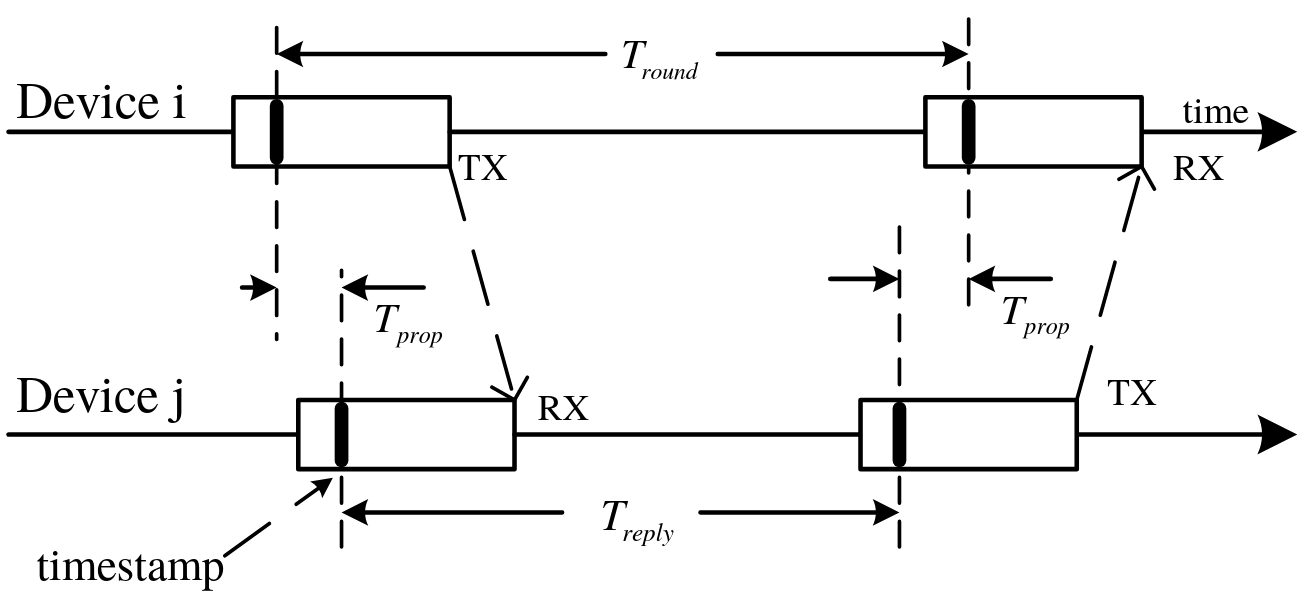
\includegraphics[width=0.69
	\linewidth]{Images/Related-Work/Single-Sided-Two-Way-Ranging-SS-TWR-5.png}
	\decoRule
	\caption[Illustration of Single-sided Two-way ranging]{Illustration of Single-sided Two-way ranging \cite{uwb-imu-gps1}}
	\label{fig:SS-TWR}
\end{figure}


Και ότι το ένα μπορεί να μεταφέρει τις πληροφορίες του στο άλλο

UWB module is set to operate at a rate of 100Hz

Each measuring interval
	dij calculate
	transmit to other nodes

% GPS
NEO-M8N GPS 5Hz.

\begin{gather*}
	r_{i,j} = r_{i, GPS} - r_{j, GPS} = r_{ij} + n_{GPS} \\
\end{gather*}


\begin{figure} [H]
	\centering
	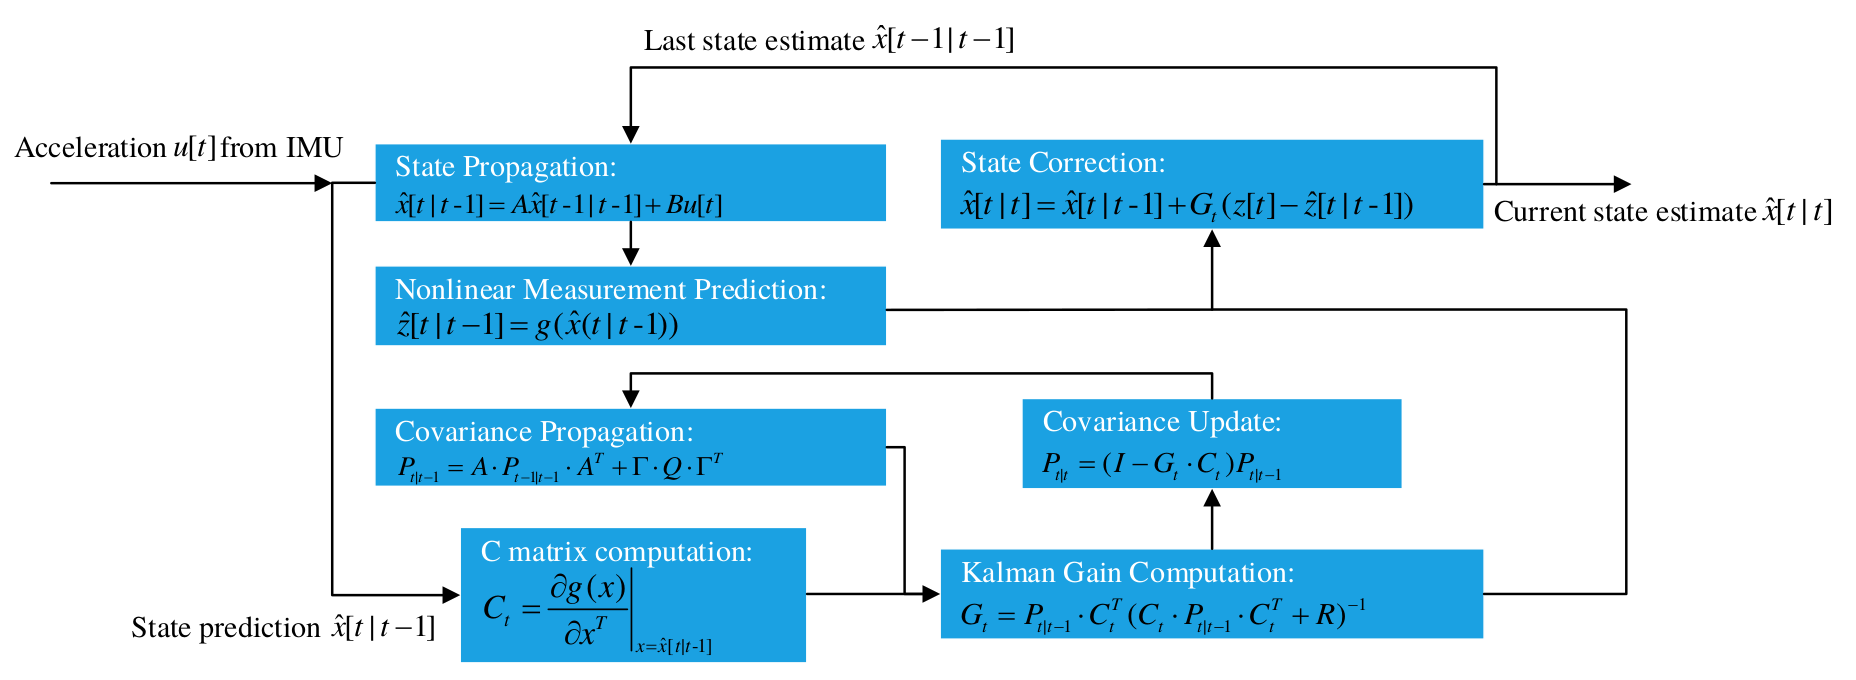
\includegraphics[width=\linewidth]{Images/Related-Work/Data-preprocessing-work-flow-using-EKF.png}
	\decoRule
	\caption[Data preprocessing work flow using EKF]{Data preprocessing work flow using EKF\cite{uwb-imu-gps1}}
	\label{fig:Data-preprocessing-work-flow-using-EKF}
\end{figure}

Θεωρούν το σύστημα ως ένα γράφο το οποίο 
το σημείο στο οποίο το σύστημα σταθεροποιηθεί θεωρείται ότι είναι το η γεωμετρία τοπολογίας των nodes
ενώ θεωρούν το σύστημα ως rigid body 

estimation problem into a non-convex optimization problem



small distance estimation error (within 0.4 m) while maintaining low
computational load

% 

of UWB pulses transmission and reception [1], and has an accuracy of less
than 10 cm UWB signals are particularly suitable for localization systems due to their high
accuracy as well as the ability to operate in Non-Line-of-Sight (NLOS)
it provides a channel for data communication and supports data transfer at a rate up to 6.8
Mbps.

First we
incorporate the UWB and the IMU measurement to reject the ranging outlier and recover the
distance between neighbors when ranging failure occurs, next we use these distance estimations
to construct a rigid body composed of these moving nodes and edges of certain length by finding
the global minimum of a non-convex function, finally the orientation of the rigid body system
is calculated using GPS coordinates of several nodes.

% ----------------------------------------------------------------


LPS methods based on Ultra-Wide Band (UWB)

Local Ad-hoc Positioning and Landing
System (LAOLa)


Components-Off-The-Shelf (COTS)
Radio based
such as Radio Fre-, WiFi [10], Zigbee [11] and
Ultra-Wideband (UWB)













% This should be the last section
\section{Thesis Approach}
TODO: As last section of this chapter
